% arara: pdflatex
% arara: pdflatex
% arara: remove: { items: [ aux , toc , log, nav, out , snm , vrb ] }
\documentclass{gittalk}

\title{Git Advanced}
\author{Andreas Gerdes}
\date{}

\usepackage{tcolorbox}
\usepackage{upquote}

% Exercises should a have a different background color to
% highlight the hands-on nature of the slide:
\newenvironment{exerciseframe}
{\setbeamercolor{background canvas}{bg=blue!20}\begin{frame}}
{\end{frame}}

% Commands could be highlighted by a different background color:
\newcommand{\hlcommand}[1]{%
\colorbox{base3}{\small \texttt{#1}}
}

\begin{document}
%============================================================================
% Titlepage

\begin{frame}
  \titlepage
  %\begin{textblock}{10}(0,-5)
  %  \includegraphics[height=40mm]{./logo.pdf}
  %\end{textblock}
\end{frame}
%============================================================================

\begin{frame}
  \frametitle{Git commands}
\begin{center}
    %\resizebox{\textwidth}{!}{
        \usetikzlibrary{positioning}

\begin{tikzpicture}
[
gitcommand/.style={rectangle, minimum width=6em, minimum height=2em, 
fill=blue!20, 
draw=blue, thick},
newgitcommand/.style={rectangle, minimum width=6em, minimum height=2em, 
fill=red!20, 
draw=red, thick},
todaygitcommand/.style={rectangle, minimum width=6em, minimum height=2em, 
fill=blue!50, 
draw=blue, thick},
]

\node [gitcommand] (config) at (0,0) {\texttt{config}};
\node [gitcommand, left = of config] (help) {\texttt{help}};
\node [gitcommand, right = of config] (init) {\texttt{init}};
\node [gitcommand, below of = help] (status) {\texttt{status}};
\node [gitcommand, below of = config] (add) {\texttt{add}};
\node [gitcommand, below of = init] (commit) {\texttt{commit}};
\node [gitcommand, below of = status] (log) {\texttt{log}};
\node [gitcommand, below of = add] (diff) {\texttt{diff}};
\node [gitcommand, below of = commit] (show) {\texttt{show}};
\node [todaygitcommand, below of = log] (clone) {\texttt{clone}};
\node [todaygitcommand, below of = diff] (pull) {\texttt{pull}};
\node [todaygitcommand, below of = show] (push) {\texttt{push}};
\node [todaygitcommand, below of = clone] (checkout) {\texttt{checkout}};
\node [gitcommand, below of = pull] (reset) {\texttt{reset}};
\node [gitcommand, below of = push] (revert) {\texttt{revert}};
\node [gitcommand, below of = checkout] (mv) {\texttt{mv}};
\node [gitcommand, below of = reset] (rm) {\texttt{rm}};
\node [newgitcommand, below of = revert] (branch) {\texttt{branch}};
\node [newgitcommand, below of = mv] (fetch) {\texttt{fetch}};
\node [newgitcommand, below of = rm] (merge) {\texttt{merge}};
\node [newgitcommand, below of = branch] (remote) {\texttt{remote}};

%  \item \texttt{clone}

\end{tikzpicture}

    %}
\end{center}
\end{frame}

\begin{frame}[fragile]
\frametitle{Course prerequisites}
\begin{tcolorbox}
Bash
\end{tcolorbox}
\vspace*{1em}
\begin{tcolorbox}[title=Text editor]
\textbf{Mac:} Text Wrangler or Text Mate 2\\
\textbf{Windows}: Notepad++\\
\textbf{Linux}: gedit, leafpad, kate, nano, vim \dots
\end{tcolorbox}
\vspace*{1em}
\begin{tcolorbox}
Git
\end{tcolorbox}
\end{frame}

\begin{exerciseframe}
\frametitle{Exercise: warm up \hfill (5 minutes)}
\begin{itemize}
  \item \texttt{mkdir -p \$HOME/Git/git\_advanced}
  \item \texttt{cd !\$}
  \item \texttt{git init}
  \item \texttt{for name in green red orange blue; do \textbackslash}\\
  \texttt{echo "\$name is a nice color." \, $>$ \$name.txt; done}\\
  \item \texttt{git add .}
  \item \texttt{git commit -m "{}Initial commit."}
  \item Modify two of the files (add a second line with things that have that color).
  \item Stage and commit the changes
  \item \texttt{git log}
\end{itemize}
\end{exerciseframe}

%============================================================================
% Table of contents

\begin{frame}
  \frametitle{Agenda}
  \tableofcontents
  \vspace*{1em}
{\footnotesize \textbf{Note: All repository pictures in this talk are taken
from the excellent Pro Git book by Scott Chacon:
\url{http://git-scm.com/book}}}
\end{frame}

%============================================================================

\section{Clone a remote repository and explore it}

\begin{frame}[fragile]
\frametitle{Clone a project}
\begin{tcolorbox}[title=git clone]
Clones a repository from some other location.\\
Many protocols are supported. Despite to \hlcommand{git init} the cloned repo
may not be empty. Use \hlcommand{git log} to see the history.
\end{tcolorbox}
\vspace*{1em}
\textbf{Example:}\\
From Github\\[0.5em]
\begin{lstlisting}[basicstyle=\footnotesize\ttfamily]
git clone https://github.com/purepitch/git_course.git
\end{lstlisting}
\end{frame}

\begin{exerciseframe}
\frametitle{Exercise: clone, log \hfill (5 minutes)}
\begin{itemize}
  \item \texttt{cd \$HOME/Git/}
  \item \texttt{git clone \textbackslash \\
         https://github.com/purepitch/git\_course.git}
  \item \texttt{cd git\_course}
  \item Explore the history of the cloned repository using\\
        \hlcommand{git log} or \hlcommand{tig}
  \item What do you find?
  \item Feel free to work (make changes, stage and commit them) \\
        in this repo!
\end{itemize}
\vspace*{1em}
\textbf{Note:} You will not be able to push your changes.
\end{exerciseframe}

%============================================================================
\section{Git in pictures}

\begin{frame}
  \frametitle{Blob, tree, commit}
\begin{center}
  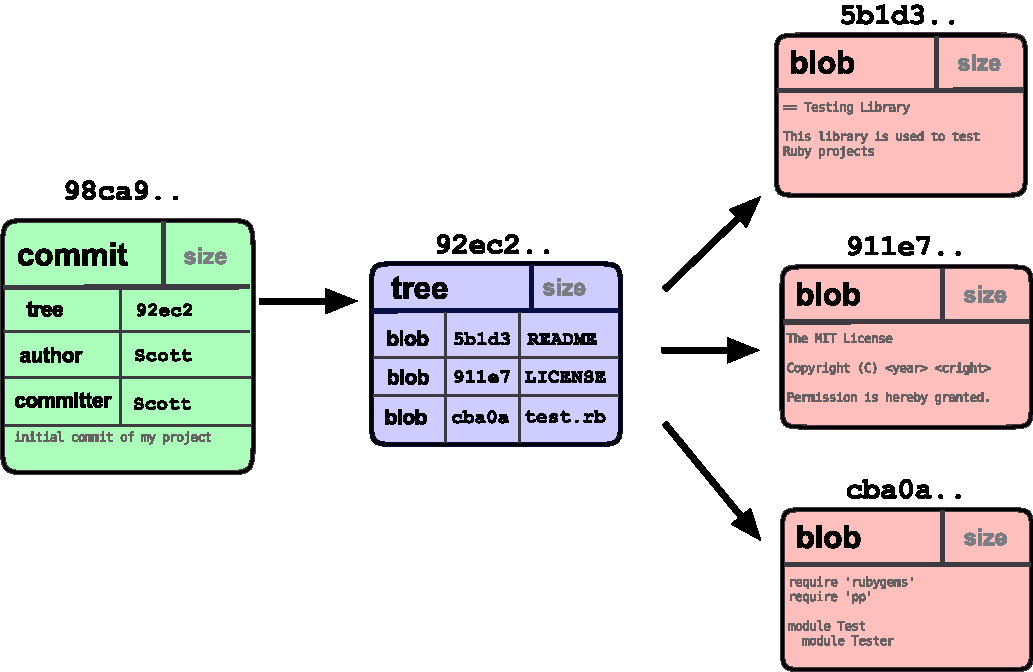
\includegraphics[width=0.9\textwidth]{./img/fig0301.pdf}
\end{center}
\end{frame}

\begin{frame}
  \frametitle{Multiple commits}
  \vspace*{2em}
\begin{center}
  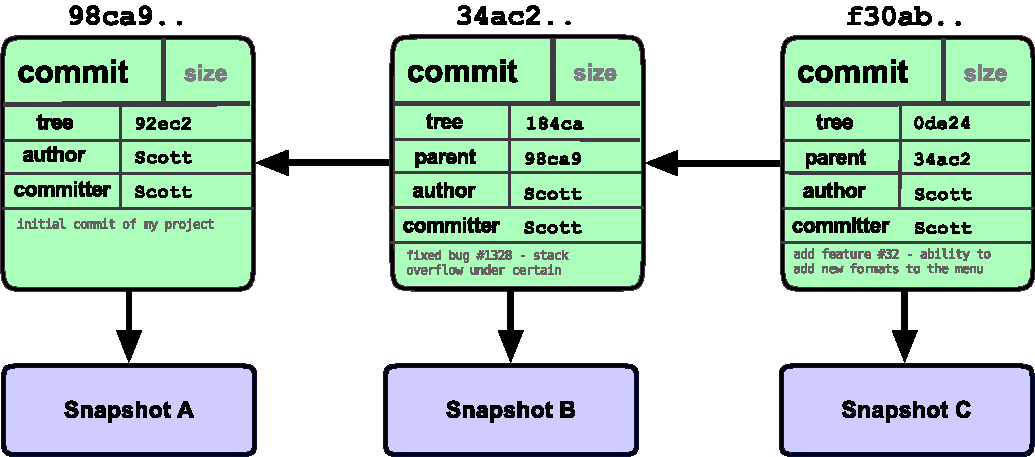
\includegraphics[width=0.9\textwidth]{./img/fig0302.pdf}
\end{center}
\end{frame}

\begin{frame}
  \frametitle{The master branch}
  \vspace*{2em}
\begin{center}
  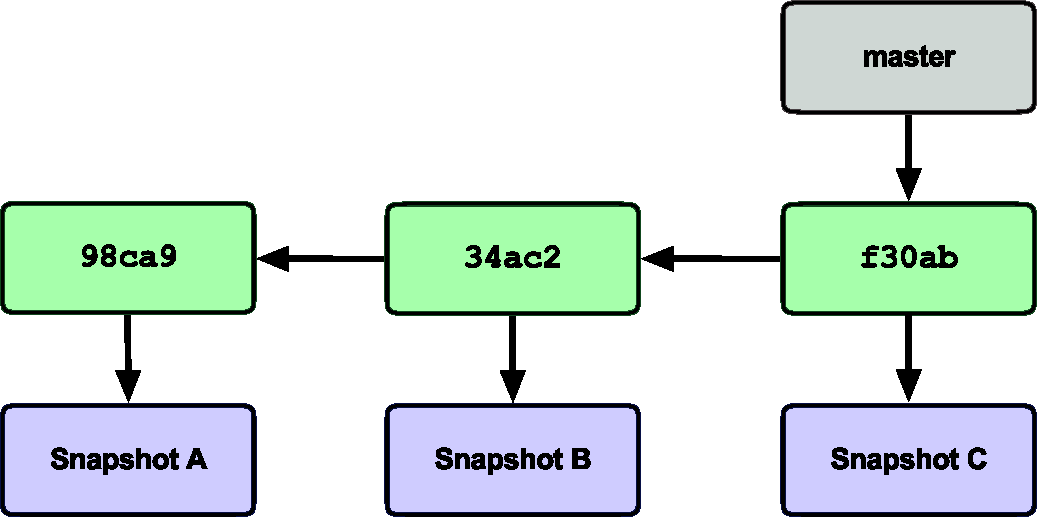
\includegraphics[width=0.6\textwidth]{./img/fig0303.pdf}
\end{center}
\end{frame}

\begin{frame}
  \frametitle{Create a new branch}
  \vspace*{2em}
\begin{center}
  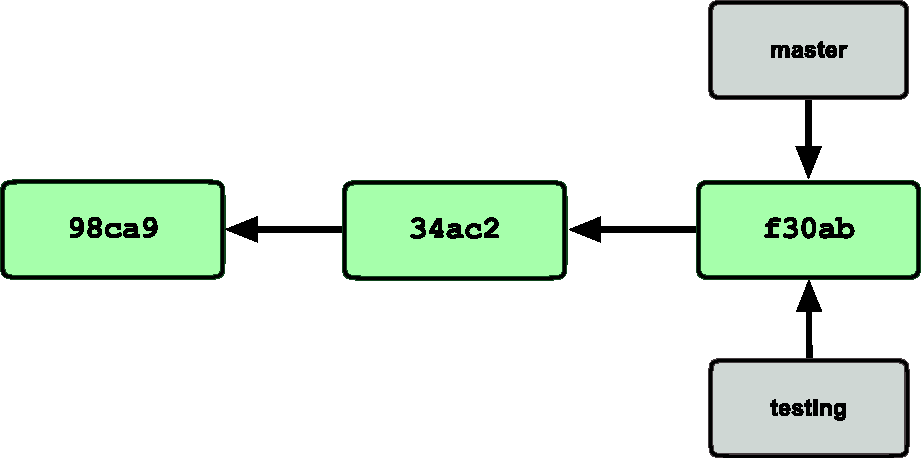
\includegraphics[width=0.6\textwidth]{./img/fig0304.pdf}
\end{center}
\end{frame}

\begin{frame}
  \frametitle{The HEAD pointer}
\begin{center}
  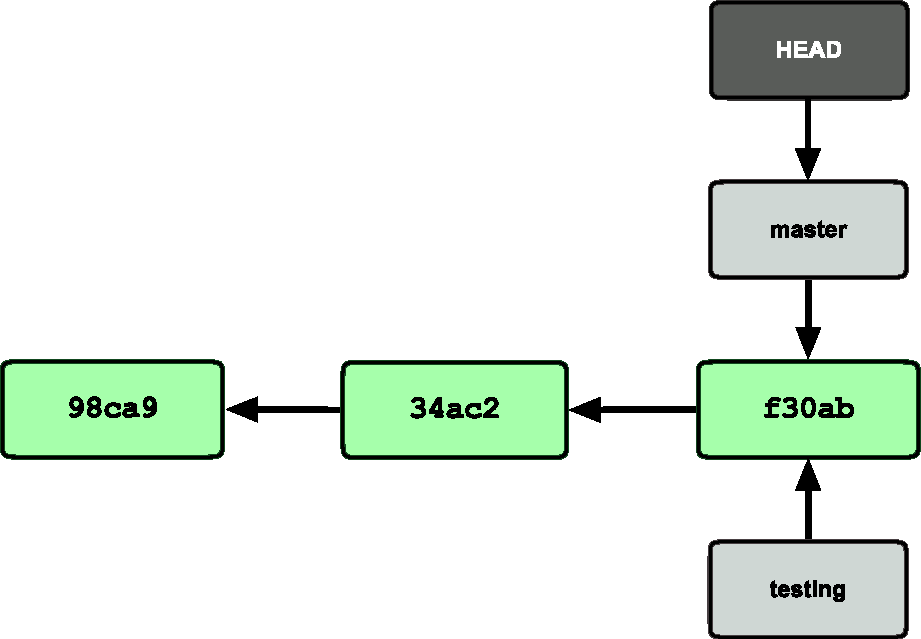
\includegraphics[width=0.6\textwidth]{./img/fig0305.pdf}
\end{center}
\end{frame}

\begin{frame}
  \frametitle{Switching branches}
\begin{center}
  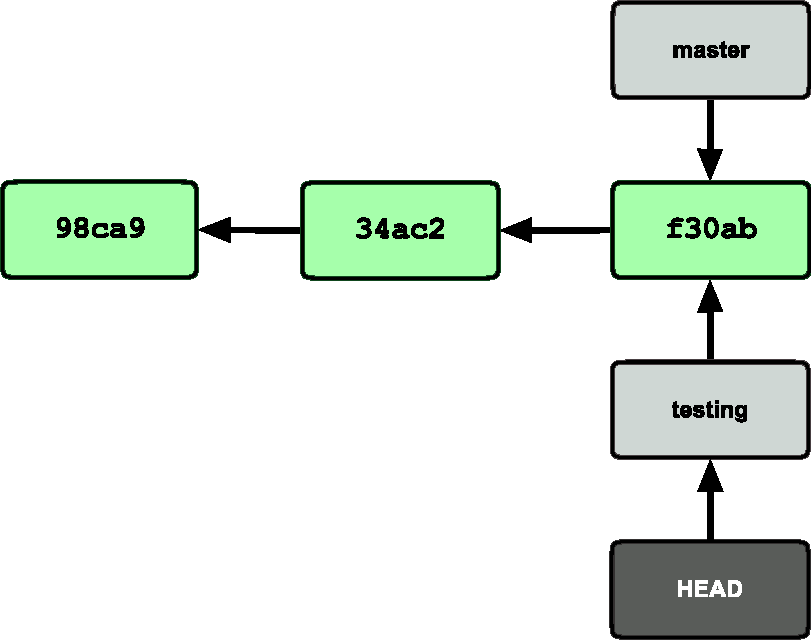
\includegraphics[width=0.6\textwidth]{./img/fig0306.pdf}
\end{center}
\end{frame}

\begin{frame}
  \frametitle{The next commit}
\begin{center}
  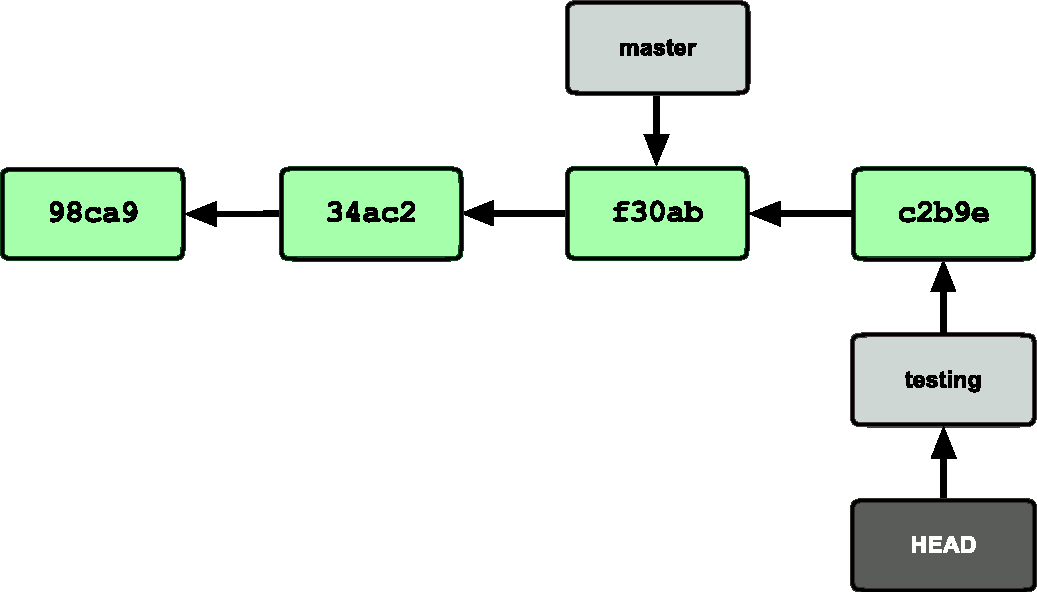
\includegraphics[width=0.8\textwidth]{./img/fig0307.pdf}
\end{center}
\end{frame}

\begin{frame}
  \frametitle{Back to master}
\begin{center}
  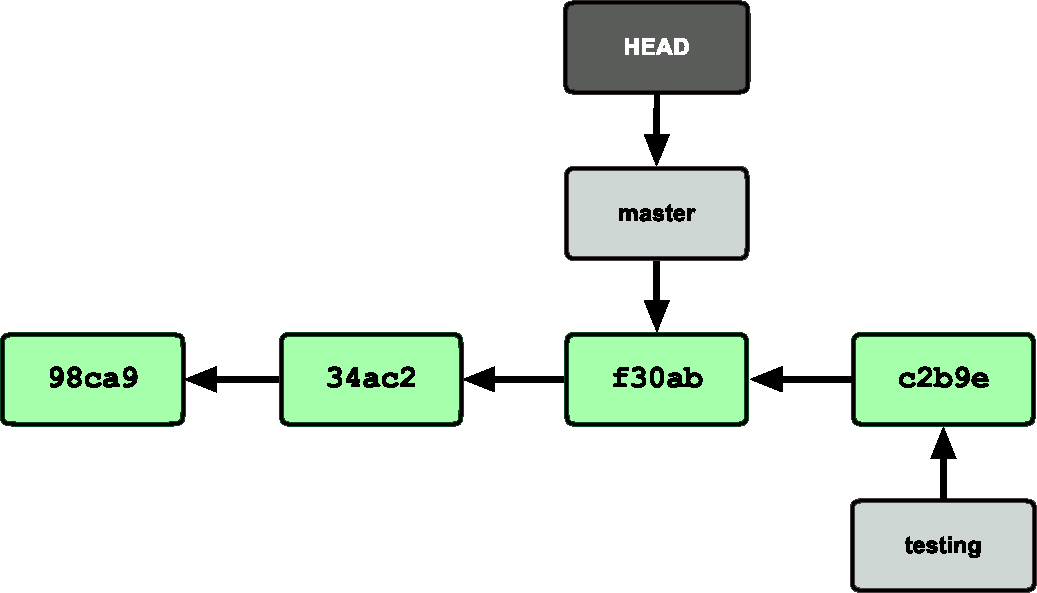
\includegraphics[width=0.8\textwidth]{./img/fig0308.pdf}
\end{center}
\end{frame}

\begin{frame}
  \frametitle{Commit in master}
\begin{center}
  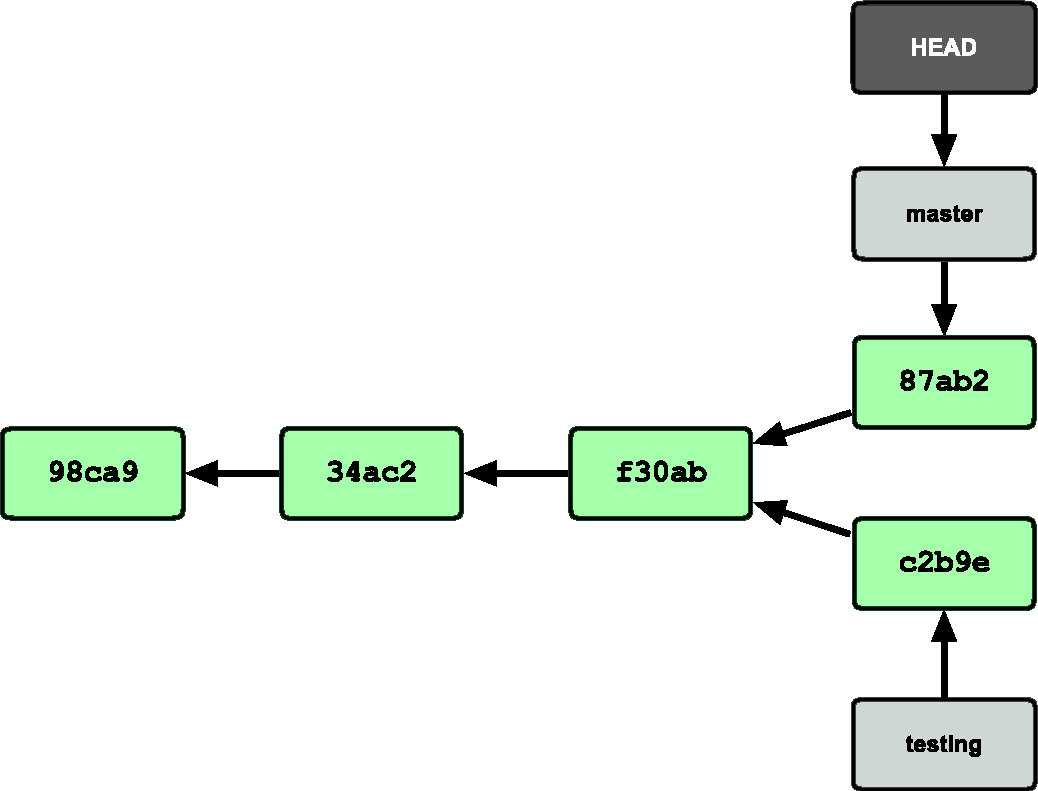
\includegraphics[width=0.8\textwidth]{./img/fig0309.pdf}
\end{center}
\end{frame}

%============================================================================
\section{Branch and merge}

\begin{frame}[fragile]
\frametitle{Branches}
\begin{tcolorbox}[title=git branch]
Shows your branches or creates (deletes) them.
\end{tcolorbox}
\vspace*{0.5em}
\begin{tcolorbox}[title=git checkout]
Checks out a branch -- or the past.
\end{tcolorbox}
\vspace*{0.5em}
Our history is not linear any more. It becomes more complex. Parallel
snapshots are possible.
\end{frame}

\begin{exerciseframe}
\frametitle{Exercise: branch, checkout \hfill (10 minutes)}
\begin{itemize}
  \item \texttt{cd \$HOME/Git/git\_advanced}
  \item Create a new branch \enquote{yellow} and checkout that branch.
  \item You can do it with\\
        \hlcommand{git branch yellow}\\
        \hlcommand{git checkout yellow}\\
        or in one step:
        \hlcommand{git checkout -b yellow}
  \item Create a file \enquote{yellow.txt} in your yellow branch (you know the content).
        Stage and commit the changes.
  \item Checkout master. Create and checkout a \enquote{red} branch and
        change the content of \enquote{red.txt} to:\\
        \texttt{red is my favorite color}
  \item Checkout master. Create and checkout a \enquote{blue} branch and
        change the content of \enquote{blue.txt} to:\\
       \texttt{blue is a cool color}
  \item Check out master and change the content of \enquote{blue.txt} to:\\
       \texttt{I am feeling blue.}
\end{itemize}
\end{exerciseframe}

\begin{frame}[fragile]
\frametitle{Merge changes into your branch}
\begin{tcolorbox}[title=git merge]
Merges changes from another branch into the one your are currently in.
\end{tcolorbox}
\vspace*{1em}
\textbf{Example:}
\begin{lstlisting}
git checkout master
git merge yellow
\end{lstlisting}
(merges branch \enquote{yellow} into master)
\end{frame}

\begin{frame}
  \frametitle{Start configuration: three branches}
\begin{center}
  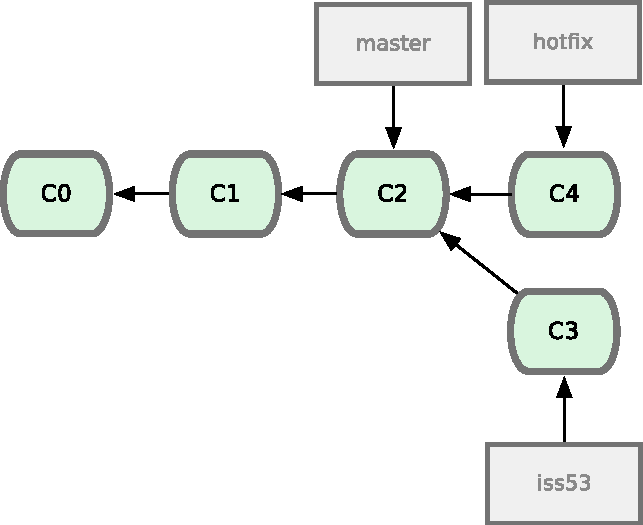
\includegraphics[width=0.6\textwidth]{./img/fig0313.pdf}
\end{center}
\end{frame}

\begin{frame}
  \frametitle{First merge: Fast forward}
\begin{center}
  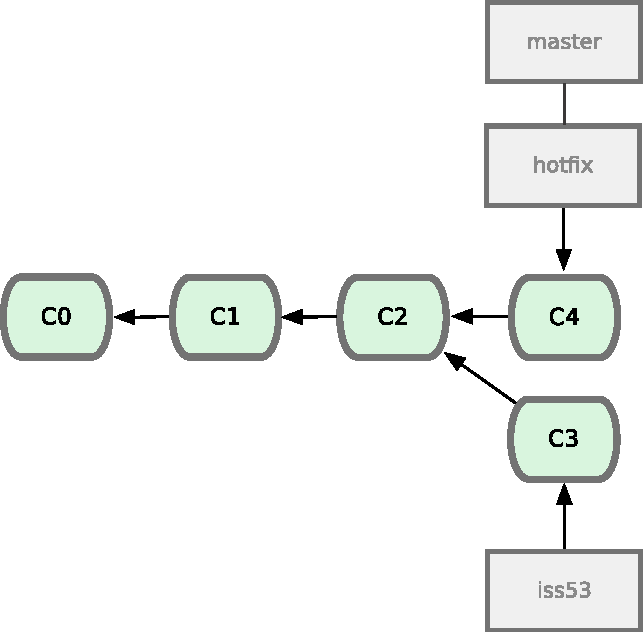
\includegraphics[width=0.6\textwidth]{./img/fig0314.pdf}
\end{center}
\end{frame}

\begin{frame}
  \frametitle{Delete hotfix and continue working}
\begin{center}
  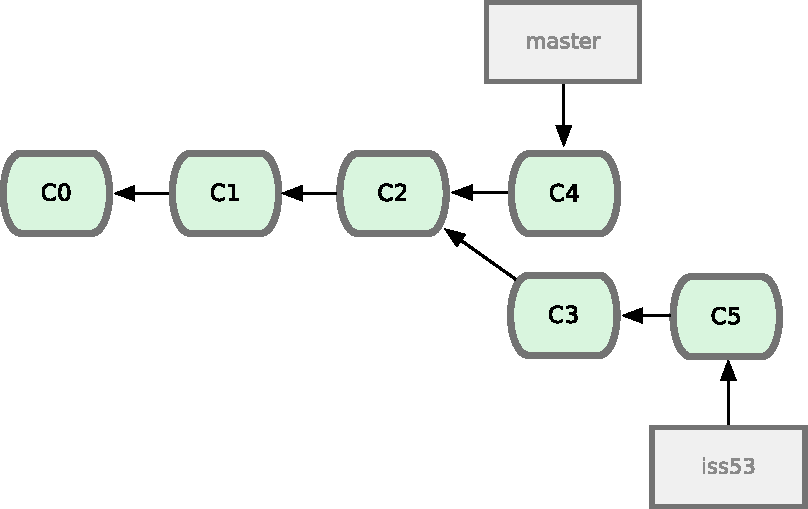
\includegraphics[width=0.75\textwidth]{./img/fig0315.pdf}
\end{center}
\end{frame}

\begin{frame}
  \frametitle{Second merge: three-way merge}
\begin{center}
  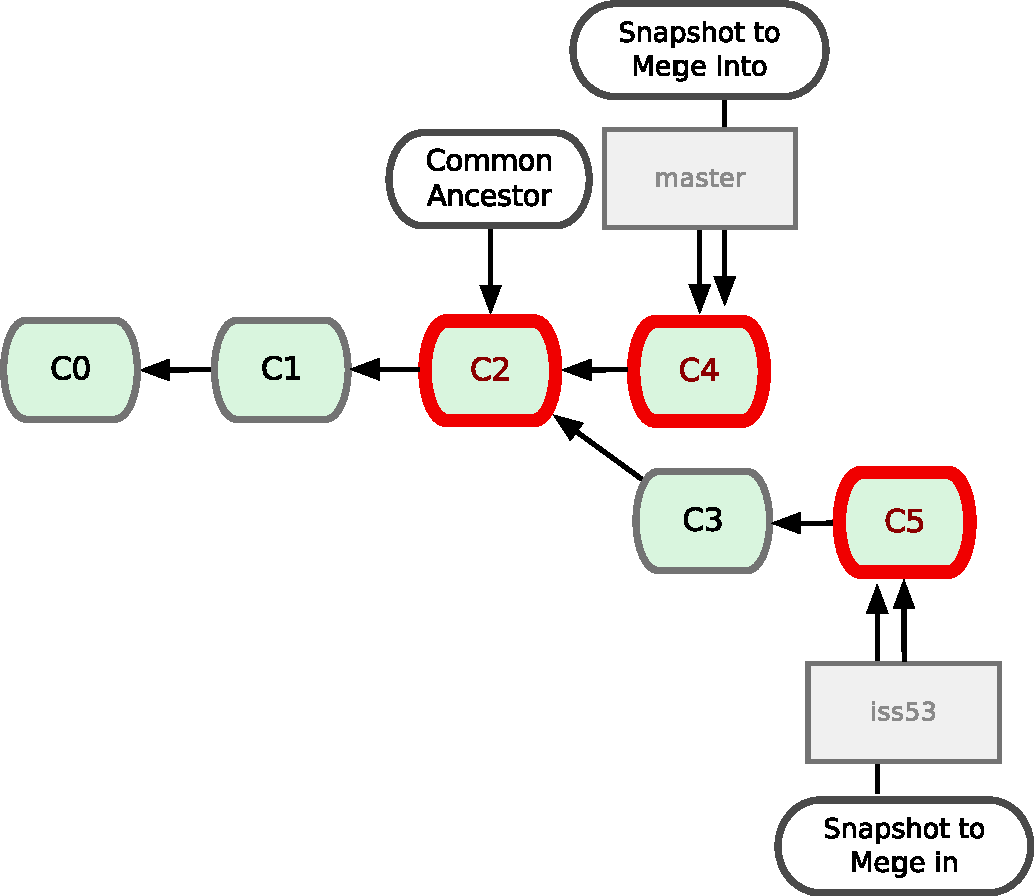
\includegraphics[width=0.75\textwidth]{./img/fig0316.pdf}
\end{center}
\end{frame}

\begin{frame}
  \frametitle{Second merge: three-way merge}
\begin{center}
  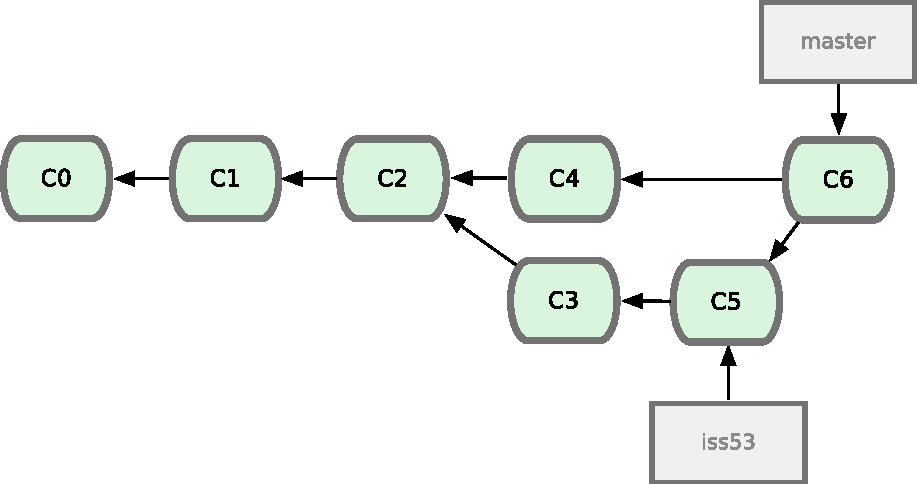
\includegraphics[width=0.75\textwidth]{./img/fig0317.pdf}
\end{center}
\end{frame}

\section{Exercises for merge conflicts}

\begin{exerciseframe}
\frametitle{Exercise: merge \hfill (10 minutes)}
\begin{itemize}
  \item \texttt{cd \$HOME/Git/git\_advanced}
  \item Checkout your master branch.
  \item Merge in your yellow branch.
  \item Merge in your red branch.
  \item Merge in your blue branch.
  \item Which merges are fast forward?
  \item Which merges are three-way merges?
  \item Do you see conflicts? In which branch? And why?
\end{itemize}
\end{exerciseframe}

%============================================================================

\section{Remotes}

\begin{frame}[fragile]
\frametitle{Working with remotes}
\begin{tcolorbox}[title=git remote]
Show, add and delete remote repositories.
\end{tcolorbox}
\vspace*{1em}
\textbf{Example 1:}
\begin{lstlisting}
git remote
\end{lstlisting}
(shows your remote, if you have any)\\[1em]
\textbf{Example 2:}
\begin{lstlisting}
git remote add andreas \
    https://github.com/purepitch/git_course.git
\end{lstlisting}
(adds a remote with the symbolic name \enquote{andreas})
\end{frame}

%============================================================================
\section{Fetch and push}

\begin{frame}[fragile]
\frametitle{Fetching from a another (remote) location}
\begin{tcolorbox}[title=git fetch]
Download objects and refs from another repository
\end{tcolorbox}
\vspace*{1em}
\textbf{Example:}
\begin{lstlisting}
git fetch andreas
\end{lstlisting}
(fetches remote content and stores it locally in the corresponding branch)
\end{frame}

\begin{frame}
\frametitle{Pushing your changes to another (remote) location}
\begin{tcolorbox}[title=git push]
Pushes local changes (commits) to the remote repo. Can only be done when all
(merge) conflicts are resolved.\\[0.5em]
Best practice:\\
Always do a pull before you try to push!
\end{tcolorbox}
\end{frame}

%============================================================================
\section{Pull}

\begin{frame}[fragile]
\frametitle{Pull changes from a remote}
\begin{tcolorbox}[title=git pull]
Fetch from and integrate with another repository or a local
branch.\\[0.5em]
Incorporates changes from a remote repository into the current branch.
In its default mode, git pull is shorthand for \hlcommand{git fetch}
followed by \hlcommand{git merge}.
\end{tcolorbox}
\end{frame}

\begin{exerciseframe}
\frametitle{Exercise: bare repository, remotes \hfill (10 minutes)}
\begin{itemize}
  \item \texttt{mkdir -p \$HOME/repositories/advanced}
  \item \texttt{cd !\$}
  \item \texttt{git init -{}-bare}
  \item \texttt{ls}
  \item $\rightarrow$ What do you see?
\pause
  \item \texttt{cd \$HOME/Git/git\_advanced}
  \item \texttt{git remote add thiscomputer \textbackslash} \\
        \texttt{file:///home/xubuntu/repositories/advanced}
  \item \texttt{git push thiscomputer master}
  \item \texttt{cd \$HOME/Git}
  \item \texttt{git clone file:///home/xubuntu/repositories/advanced}
\end{itemize}
\end{exerciseframe}

\begin{exerciseframe}
\frametitle{Exercise: pull vs.\ fetch and merge \hfill (10 minutes)}
\begin{itemize}
  \item \texttt{cd \$HOME/Git/git\_course}
  \item I have made changes on the server. Pull them.
  \item How do you see what has changed?
  \item Remove the first line in \enquote{green.txt}, stage and commit the change.
\pause
  \item Again some changes. Pull them.\\
        (You should have a conflict now. Why?)
\pause
  \item Another change on the server.
  \item This time, do it in two steps:
  \item 1) \hlcommand{git fetch}
  \item Did anything happen?
  \item Can you show me the change? How?
  \item 2) \hlcommand{git merge remote/origin/master}
\end{itemize}
\end{exerciseframe}

\section{Deleting a remote branch}

\begin{frame}
    \frametitle{Deleting a remote branch once you are finished with it}

\begin{lstlisting}
    # as of git 1.7.0
    git push origin --delete <branch_name>
    # previously
    git push origin :<branch_name>
\end{listlisting}
\end{frame}

\section{Topics not discussed}

\begin{frame}
\frametitle{What we did not discuss}
\begin{itemize}
  \item \hlcommand{git stash}
  \item \hlcommand{git tag}
  \item \hlcommand{git rebase}
  \item Stage only parts of a file: \texttt{git add -p}
\end{itemize}
\end{frame}

\section{Further reading}

\begin{frame}
\frametitle{Further reading}
\begin{itemize}
    \item \href{http://jwiegley.github.io/git-from-the-bottom-up/}{Git from the Bottom Up}
    \item \href{http://tbaggery.com/2008/04/19/a-note-about-git-commit-messages.html}
               {A note about commit messages}
\end{itemize}
\end{frame}

\end{document}

\begin{frame}
\frametitle{Agenda}
\begin{itemize}

  \item \texttt{git stash}
  \item \texttt{git rebase}
  \item git tag?
\end{itemize}
\end{frame}

\begin{frame}
    \frametitle{Extras}
    \begin{itemize}
        \item Graphically display commits and branches in the terminal
        \item \texttt{git log --graph --oneline --decorate --all}
    \end{itemize}
\end{frame}

% vim: shiftwidth=4 expandtab:
